\documentclass[tikz,border=10pt]{standalone}
\usepackage[utf8]{inputenc}
\usepackage[T1]{fontenc}
\usepackage{lmodern}
\usetikzlibrary{arrows.meta,positioning,calc}
\definecolor{navy}{HTML}{15324B}
\definecolor{blue}{HTML}{2F80C1}
\definecolor{lightblue}{HTML}{E7F2F8}
\definecolor{orange}{HTML}{E8873A}
\definecolor{green}{HTML}{3B8F72}
\tikzset{
  pointlabel/.style={font=\sffamily\bfseries\normalsize,text=navy},
  paneltitle/.style={draw=navy,rounded corners=3pt,fill=white,
    text=navy,font=\sffamily\bfseries,align=center,inner sep=6pt},
  principle/.style={draw=blue,rounded corners=4pt,fill=lightblue,
    text=navy,font=\sffamily\bfseries,align=center,inner xsep=12pt,inner ysep=7pt}
}
\begin{document}
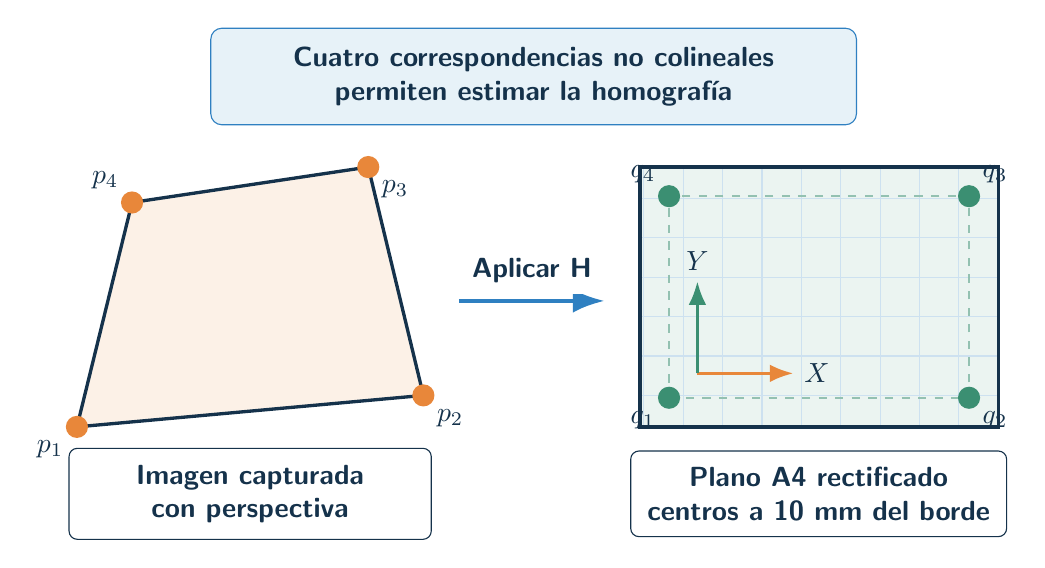
\begin{tikzpicture}[font=\sffamily]
  \node[principle,minimum width=8.2cm] at (6.1,5.05)
    {Cuatro correspondencias no colineales\\permiten estimar la homografía};

  \coordinate (p1) at (0.3,0.6);
  \coordinate (p2) at (4.7,1.0);
  \coordinate (p3) at (4.0,3.9);
  \coordinate (p4) at (1.0,3.45);
  \fill[orange!12] (p1)--(p2)--(p3)--(p4)--cycle;
  \draw[navy,very thick] (p1)--(p2)--(p3)--(p4)--cycle;
  \foreach \p in {p1,p2,p3,p4}{\fill[orange] (\p) circle (4pt);}
  \node[pointlabel,below left=2pt of p1] {$p_1$};
  \node[pointlabel,below right=2pt of p2] {$p_2$};
  \node[pointlabel,below right=2pt of p3] {$p_3$};
  \node[pointlabel,above left=2pt of p4] {$p_4$};
  \node[paneltitle,minimum width=4.6cm] at (2.5,-0.25)
    {Imagen capturada\\con perspectiva};

  \draw[-{Latex[length=4mm]},blue,ultra thick] (5.15,2.2)--(7.0,2.2);
  \node[text=navy,font=\sffamily\bfseries,fill=white,inner sep=4pt] at (6.08,2.58)
    {Aplicar H};

  \coordinate (C1) at (7.45,0.6);
  \coordinate (C3) at (12.0,3.9);
  \coordinate (q1) at (7.82,0.97);
  \coordinate (q2) at (11.63,0.97);
  \coordinate (q3) at (11.63,3.53);
  \coordinate (q4) at (7.82,3.53);
  \fill[green!10] (C1) rectangle (C3);
  \draw[step=0.5cm,blue!24] (C1) grid (C3);
  \draw[navy,very thick] (C1) rectangle (C3);
  \draw[green!55,dashed,thick] (q1)--(q2)--(q3)--(q4)--cycle;
  \foreach \p in {q1,q2,q3,q4}{\fill[green] (\p) circle (4pt);}
  \node[pointlabel,below left=2pt of q1] {$q_1$};
  \node[pointlabel,below right=2pt of q2] {$q_2$};
  \node[pointlabel,above right=2pt of q3] {$q_3$};
  \node[pointlabel,above left=2pt of q4] {$q_4$};
  \draw[orange,very thick,-{Latex[length=3mm]}] (8.18,1.28)--(9.40,1.28)
    node[right,pointlabel] {$X$};
  \draw[green,very thick,-{Latex[length=3mm]}] (8.18,1.28)--(8.18,2.45)
    node[above,pointlabel] {$Y$};
  \node[paneltitle,minimum width=4.6cm] at (9.72,-0.25)
    {Plano A4 rectificado\\centros a 10 mm del borde};
\end{tikzpicture}
\end{document}
